\lesson{Hello world}

Die erste Lektion beschäftigt sich alleine mit der Frage, was eigentlich eine
Programmiersprache überhaupt ist und wie wir den Computer dazu bringen können,
daraus etwas zu machen, was er ausführen kann.  In guter alter
Programmiertradition tun wir das an dem simpelsten aller Programme: Einem, was
einfach nur ein „Hallo Welt!“ ausgibt.

Wie bringen wir also den Computer dazu, diese Ausgabe zu generieren? Dass er
keine natürliche Sprache versteht, sollte klar sein - intern besteht er aus
lauter Transistoren (wenn ihr nicht wisst, was das ist, denkt an winzige
Schalter), die nur die Zustände „an“ und „aus“ kennen, wir müssen also die
Anweisung „gebe Hallo Welt aus“ in ein Format übersetzen, was nur „an“ und
„aus“ benutzt.

Früher wurde genau dies benutzt - meistens über Lochkarten, die vom Computer
gelesen wurden, „ein Loch“ war dann zum Beispiel ein „an“ und „kein Loch“ war
„aus“, so wurde dann das Programm in Reihen angeordnet und jede Reihe entsprach
einem Befehl oder einem Parameter für diesen Befehl.  Dieses Format nennt sich
„Maschinensprache“ und ist immer noch das, was wir heute dem Computer
übergeben, nur, dass wir keine Lochkarten mehr benutzen, sondern Dateien, in
denen lange Ströme von codierten 0en und 1en stehen.

Nun kann man sich vorstellen, dass es ganz schön anstrengend ist, ein
umfangreiches Programm in 0en und 1en zu beschreiben. Deswegen benutzt man
heutzutage so genannte Hochsprachen, um Programme zu beschreiben. Wir
beschreiben also den Programmablauf in einer von Menschen lesbaren und
verstehbaren Sprache -- wir benutzen hier \Cpp.  Die Programmbeschreibung in
\Cpp legen wir dabei in einer Textdatei ab, meistens hat diese die Endung
\texttt{.cpp}.

Diese Beschreibung des Programms übergeben wir dann an einen \emph{Compiler},
der daraus dann Maschinencode generiert, den wir wiederum dem Computer zur
Ausführung geben können.  Der Compiler für \Cpp, den wir in diesem Kurs
benutzen wollen, heißt \texttt{g++}.

Dem Compiler übergeben wir die zu kompilierende Datei als Parameter, sowie den
Namen der Ausgabedatei (mit einem \texttt{-o} davor).

Nachdem \texttt{g++} uns also ein Maschinencodefile \texttt{datei} erzeugt hat,
können wir es zur Ausführung bringen. Wir tun das, indem wir in einem Terminal
\texttt{./datei} eingeben, also einen Punkt, ein Slash und dann den Dateinamen.

% TODO: Buttugly, but well...
\begin{center}
    \resizebox{\textwidth}{!}{
        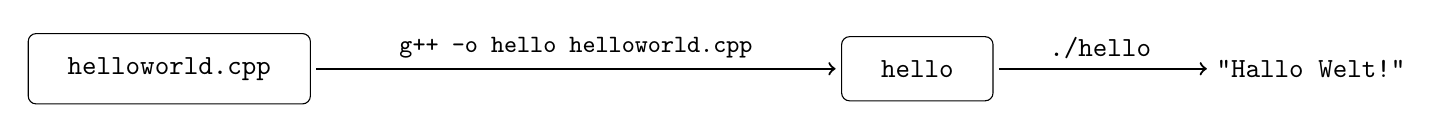
\begin{tikzpicture}
            \node (nHelloWorldCpp) [ shape=rectangle, rounded corners = 0.1cm, draw=black, inner xsep=0.5cm, inner ysep = 0.3cm ] {\texttt{helloworld.cpp}};
            \node (nHello) [ right of = nHelloWorldCpp, node distance = 9.5cm, shape=rectangle, rounded corners = 0.1cm, draw = black, inner xsep = 0.5cm, inner ysep = 0.3cm ] {\texttt{hello}};
            \draw [->, thick, shorten >= 2pt, shorten <= 2pt ] (nHelloWorldCpp) -- (nHello) node [ midway, above, font = \small ] { \texttt{g++ -o hello helloworld.cpp}} ;
            \node (nOutput) [ right of = nHello, node distance = 5cm, shape=rectangle ] {\texttt{"Hallo Welt!"}};
            \draw [->, thick, shorten <= 2pt] (nHello) -- (nOutput) node [ midway, above ] {\texttt{./hello}};
        \end{tikzpicture}
    }
\end{center}

\textbf{Praxis:}
\begin{enumerate}
    \item Öffnet ein Terminal, ihr findet dies im Anwendungsmenü unter „System“
    \item Wechselt in das Verzeichnis \texttt{vorkurs/lektion1}, indem ihr
        \texttt{cd vorkurs/lektion1} eingebt und enter drückt.
    \item In diesem Verzeichnis liegt eine Datei \texttt{helloworld.cpp}.
        Benutzt \texttt{g++}, um diese zu einer Datei \texttt{hello} zu
        kompilieren.
    \item Führt die Datei \texttt{hello} aus.
\end{enumerate}

\inputcpp{helloworld.cpp}

\textbf{Spiel:}

Ihr könnt nun versuchen, den Quellcode selbst zu verändern und damit ein wenig
herumzuspielen. Öffnet dazu einen Editor (im Anwendungsmenü findet ihr z.B.
gedit) und öffnet die Datei \texttt{vorkurs/lektion1/helloworld.cpp}. Denkt
daran, nach jeder Änderung die Datei zu speichern und im Terminal neu zu
kompilieren und auszuführen.

Dinge, die ihr ausprobieren könntet sind zum Beispiel:
\begin{enumerate}
    \item Was passiert, wenn ihr „Hello world!“ in etwas anderes ändert?
    \item Was passiert, wenn ihr die erste Zeile löscht (der Originalquellcode
        ist in diesem pdf enthalten, ihr könnt sie also später wieder
        herstellen)?
    \item Was passiert, wenn ihr das „\verb|<< std::endl|“ löscht?
    \item Wie könnte man mehrere Sätze ausgeben? Wie könnte man mehrere Zeilen
        ausgeben?
\end{enumerate}
